\subsection{Proportion of individuals within target}\label{sec:proportion_within_target}

Another performance measure that is taken into consideration is the proportion 
of individuals whose waiting and service times are within a specified 
time target \(t\).
Similar to section \ref{sec:waiting_time} three formulas are needed for this 
performance measure.

The proportion of type 1 individuals within a time target:

\begin{equation}\label{eq:proportion_within_target_type_1}
    P(X^{(1)} < t) = \frac{\sum_{(u,v) \in S_A^{(1)}} P(X_{(u,v)}^{(1)} < t) 
    \pi_{u,v} }{\sum_{(u,v) \in S_A^{(1)}} \pi_{u,v}}
\end{equation}

The proportion of type 2 individuals within a time target remains as:

\begin{equation}\label{eq:proportion_within_target_type_2}
    P(X^{(2)} < t) = \frac{\sum_{(u,v) \in S_A^{(2)}} P(X_{(u,v)}^{(2)} < t) 
    \pi_{u,v} }{\sum_{(u,v) \in S_A^{(2)}} \pi_{u,v}}
\end{equation}

The overall proportion individuals within a time target (where \(P_{L'_1}\) and 
\(P_{L'_1}\) are defined in (\ref{eq:proportion_of_accepting_individuals})):

\begin{equation}\label{eq:overall_proportion_within_target}
    P(X < t) = \frac{\lambda_1 P_{L'_1}}{\lambda_2 P_{L'_2}+\lambda_1 P_{L'_1}} 
    P(X^{(1)} < t) + \frac{\lambda_2 P_{L'_2}}{\lambda_2 P_{L'_2} + 
    \lambda_1 P_{L'_1}} P(X^{(2)} < t) 
\end{equation}

Here \(P(X_{(u,v)}^{(1)})\) and \(P(X_{(u,v)}^{(2)})\) are defined as the
proportion of individuals within the time target \(t\) when starting from state 
\((u,v)\).
These expression can be calculated by:

\begin{equation}\label{eq:proportion_within_target_type_1_from_state}
    P(X_{(u,v)}^{(1)} < t) = 
    \begin{cases}
        1 - \sum_{i=0}^{v-1} \frac{1}{i!} e^{-\mu t} (\mu t)^i, 
            & \textbf{if } C = 1 \\
            & \textbf{and } v>1 \\
        1 - (\mu C)^{v-C} \mu  
            \sum_{k=1}^{\mid \vec{r} \mid} \sum_{l=1}^{r_k}
            \frac{\Psi_{k,l}(-\lambda_k)t^{r_k - l} 
            e^{-\lambda_k t}}{(r_k - l)! (l - 1)!},
            & \textbf{if } C > 1 \\
            & \textbf{and } v > C \\
        1 - e^{-\mu t},  & \textbf{if } v \leq C
    \end{cases}
\end{equation}

\noindent
where \(\vec{r}=(v - C, 1)\), \(\vec{\lambda}=(C \mu, \mu)\) and 
\(\lambda_0 = 0, r_0\) = 1. 

\begin{equation}\label{eq:proportion_within_target_type_2_from_state}
    P(X_{(u,v)}^{(2)} < t) = 
    \begin{cases}
        1 - \sum_{i=0}^{\min(v,T)-1} \frac{1}{i!} e^{-\mu t} (\mu t)^i,  
            & \textbf{if } C = 1 \\ 
            & \textbf{and } v, T > 1 \\
        1 - (\mu C) ^ {\min(v,T) - C} \mu  
        \sum_{k=1}^{\mid \vec{r} \mid} & \textbf{if } C > 1 \\
        \qquad \times \sum_{l=1}^{r_k}
        \frac{\Psi_{k,l}(-\lambda_k)t^{r_k - l} 
        e^{-\lambda_k t}}{(r_k - l)! (l - 1)!}, 
            & \textbf{and } v, T  > C\\
        1 - e^{-\mu t}, & \textbf{if } v \leq C \\ 
            & \textbf{or } T \leq C \\
    \end{cases}
\end{equation}

\noindent
where \(\vec{r}=(\min(v, T) - C, 1)\), \(\vec{\lambda}=(C \mu, \mu)\) and
\(\lambda_0 = 0, r_0 = 1\).


The function \(\Psi_{k,l}\) used in equations 
(\ref{eq:proportion_within_target_type_1_from_state}) and 
(\ref{eq:proportion_within_target_type_2_from_state}) is defined as:

\begin{equation}
    \Psi_{k,l}(t) = 
    \begin{cases} 
        \frac{(-1)^{l} (l-1)!}{\lambda_2} \left[\frac{1}{t^l} - \frac{1}
        {(t + \lambda_2)^l}\right] , & k=1 \\
        - \frac{1}{t (t + \lambda_1)^{r_1}}, & k=2
    \end{cases} \nonumber \\
\end{equation}

Refer to appendix \ref{sec:appendix_mean_proportion} for a more in-depth 
explanation of the origins of equations 
(\ref{eq:proportion_within_target_type_1}) - 
(\ref{eq:proportion_within_target_type_2_from_state}).

Figures \ref{fig:markov_vs_des_proportion_comparison_1},
\ref{fig:markov_vs_des_proportion_comparison_2} and 
\ref{fig:markov_vs_des_proportion_comparison_overall} show a comparison of the
mean proportion of individuals within target when using Markov chains and 
discrete event simulation (appendix~\ref{sec:appendix_des}).
The simulation was ran 100 times and the recorded proportions at each iteration 
is used to populate the violin plots.

\begin{figure}[H]
    \centering
    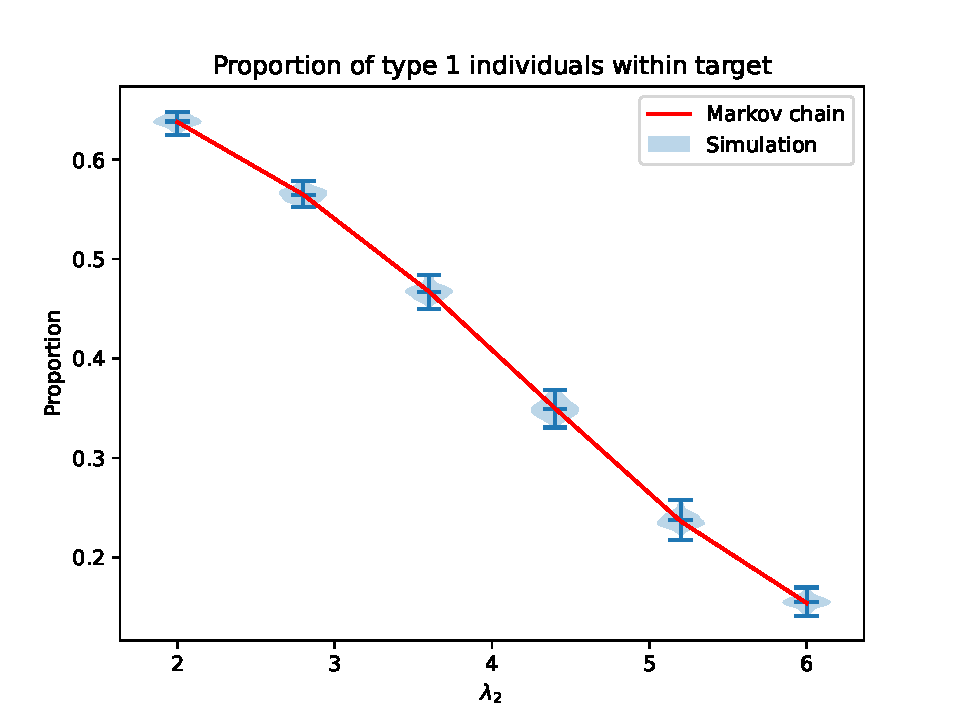
\includegraphics[width=.8\textwidth]{imgs/proportion_within_target_comparison/proportion_1.pdf}
    \caption{
        Comparison of proportion within target time for type 1 individuals 
        between values obtained from the Markov chain formulas and values 
        obtained from simulation. 
    }
    \label{fig:markov_vs_des_proportion_comparison_1}
\end{figure}

\begin{figure}[H]
    \centering
    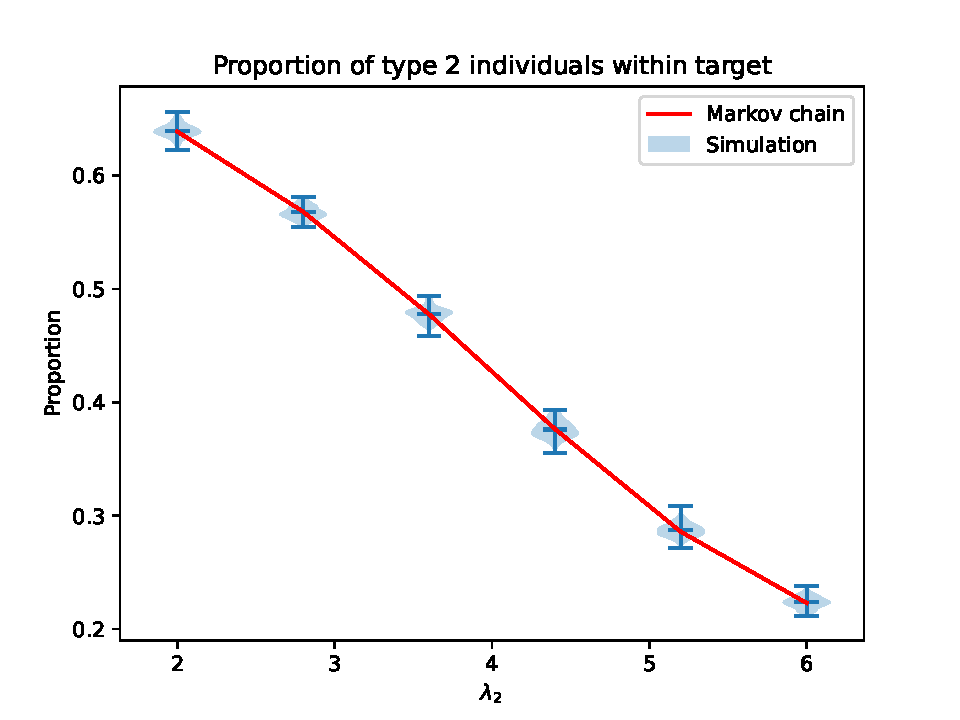
\includegraphics[width=.8\textwidth]{imgs/proportion_within_target_comparison/proportion_2.pdf}
    \caption{
        Comparison of proportion within target time for type 2 individuals 
        between values obtained from the Markov chain formulas and values 
        obtained from simulation. 
    }
    \label{fig:markov_vs_des_proportion_comparison_2}
\end{figure}

\begin{figure}[H]
    \centering
    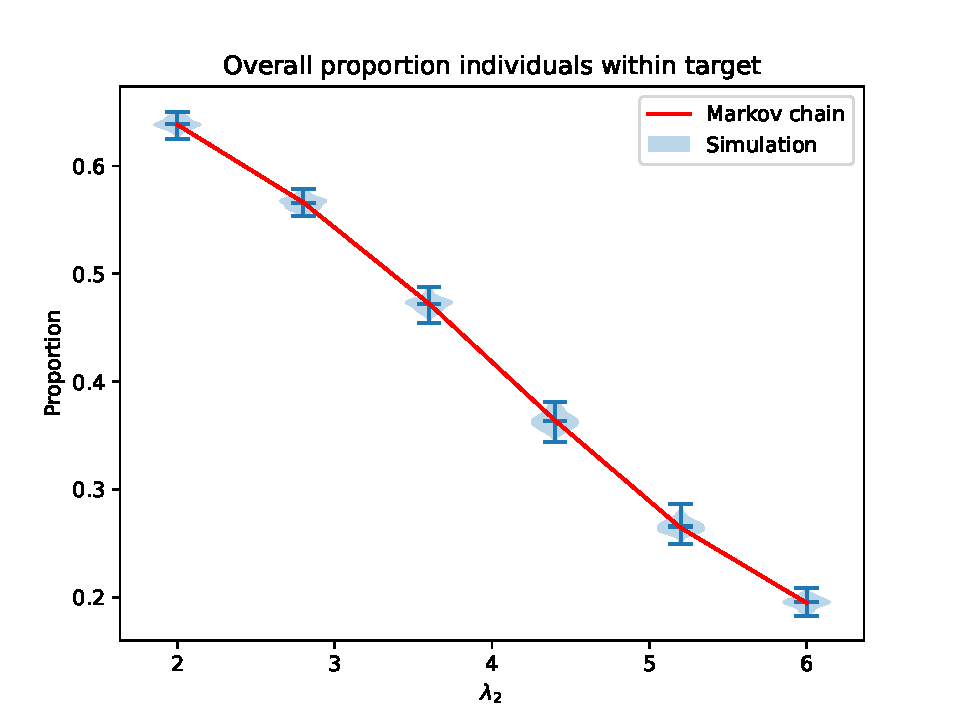
\includegraphics[width=.8\textwidth]{imgs/proportion_within_target_comparison/proportion_overall.pdf}
    \caption{
        Comparison of proportion within target time for both type of 
        individuals between values obtained from the Markov chain formulas 
        and values obtained from simulation. 
    }
    \label{fig:markov_vs_des_proportion_comparison_overall}
\end{figure}
